% Illustration of data -> text for requirements analysis

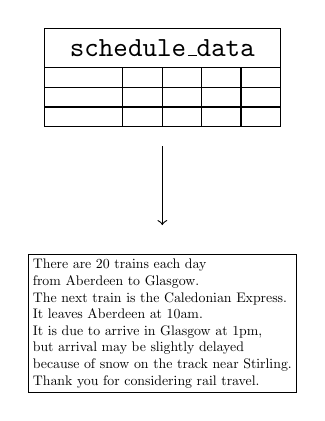
\begin{tikzpicture}

\draw (0, 1.00) -- (3, 1.00);
\draw (0, 1.25) -- (3, 1.25);
\draw (0, 1.50) -- (3, 1.50);
\draw (0, 1.75) -- (3, 1.75);
\draw (0, 2.25) -- (3, 2.25);

\draw (0.0, 1.00) -- (0.0, 2.25);
\draw (1.0, 1.00) -- (1.0, 1.75);
\draw (1.5, 1.00) -- (1.5, 1.75);
\draw (2.0, 1.00) -- (2.0, 1.75);
\draw (2.5, 1.00) -- (2.5, 1.75);
\draw (3.0, 1.00) -- (3.0, 2.25);

\node at (1.5, 2) {\texttt{schedule\_data}};

\draw [->] (1.5, 0.75) -- (1.5, -0.25);

\node [rectangle, draw, align=left, scale=0.5] at (1.5, -1.5) {
	There are 20 trains each day\\
	from Aberdeen to Glasgow.\\
	The next train is the Caledonian Express.\\
	It leaves Aberdeen at 10am.\\
	It is due to arrive in Glasgow at 1pm,\\
	but arrival may be slightly delayed\\
	because of snow on the track near Stirling.\\
	Thank you for considering rail travel.
};

\end{tikzpicture}